\section{Functional Requirements}

Given all the assumptions, domain properties and constraints from \underline{\autoref{cap:Intro}}, these functional requirements can be stated, listed by the goal they fulfill

\begin{itemize}
\item \textbf{[GOAL1]} Driver must log in the system 
	\begin{itemize}
	\item The system must check if the provided user exists and if the provided password matches
	\item The system must provide further access only if the user is logged
	\end{itemize}
\item \textbf{[GOAL2]} Allow drivers to reserve a Vehicle up to one hour before they pick it up
	\begin{itemize}
	\item The system must access driver GPS position or use a user-provided position to recommend the best vehicle to choose
	\item The system must check if the user is logged in and if it is not a blocked driver
	\item The system must check that the user has no other active reservation 
	\item The system must check payment service by pre-authorizing a payment of a fixed amount (to be defined)
	\item The system must reserve the chosen vehicle, i.e. no other user is allowed to reserve the Vehicle until it is available again, once the payment is done. The vehicle is considered available again in case of: drop off, cancel registration, one hour passed from the reservation without any driver interaction
	\end{itemize}
\item \textbf{[GOAL3]} Allow drivers to open the reserved Vehicle
	\begin{itemize}
	\item The system must check if the user is nearby the reserved Vehicle to open it
	\item The system must be able to open the Vehicle remotely, only if the user effectively reserved it and is nearby
	\end{itemize}
\item \textbf{[GOAL4]} Allow drivers to pay correctly for the service
	\begin{itemize}
	\item The system must log the whole drive by the driver (elapsed time, driven km)
	\item The system must compute the amount the driver must pay for the service. The total amount due is computed by calculating a base amount depending on the Drive duration at the current fares (� per minute), and applying discounts, as shown in Table 3.1 .
	\item The system must request a payment of the correct amount 
	\end{itemize}
	
\begin{table}
  \centering
    \begin{tabular}{| l | l |}
    \hline
    \textbf{Action} & \textbf{Discount} \\ \hline
    Driver took more than 2 passengers on the Drive & -10\% \\ \hline
    Vehicle is left with 50\% battery or more & -20\% \\ \hline
    Vehicle is left recharging & -30\% \\ \hline
    Vehicle is left far from charging station (3km) or with less than 20\% battery & +30\% \\ \hline
    \end{tabular}
  \caption{Discounts}
\end{table}

\item \textbf{[GOAL5]} Allow drivers to cancel a reservation
	\begin{itemize}
	\item The system must be able to cancel a reservation if the driver asks it, given that the reservation has not exceed the 1 hour limit, without making him pay
	\end{itemize}
\item \textbf{[GOAL50]} Worker must log in the system
	\begin{itemize}
	\item The system must check if the provided worker id exists and if the password matches
	\item The system must provide further access only to logged workers
	\end{itemize}
\item \textbf{[GOAL51]} Dispatch tasks to workers
	\begin{itemize}
	\item The system must be able to create a new task. The new task can be created from the administration console or generated automatically by a set of pre-defined rules (e.g. maintenance, usage balance)
	\item The system must select the nearest available worker and assign him the task
	\item The system must notify to the selected user that a new task has been assigned to him
	\end{itemize}
\item \textbf{[GOAL52]} Allow workers to get informations about an assigned task
	\begin{itemize}
	\item The system must provide through the PowerEniWorker App all the needed information for the Worker. These include the GPS position of the Vehicle, the reported issue and additional information the user could have provided
	\end{itemize}
\item \textbf{[GOAL53]} Allow workers to open and control the assigned Vehicle
	\begin{itemize}
	\item The System, during the assignment of a Task, gives to the chosen Worker the complete control of the Vehicle, i.e. normal actions (turn on/off engine, lock/unlock) but also priviliged actions (open hood, access maintenance interfaces, e.g. OBD)
	\end{itemize}
\item \textbf{[GOAL54]} Allow workers to update the state of the task (assigned, in progress, done)
	\begin{itemize}
	\item The System must provide, through the PowerEniWorker App, buttons to change the state of the assigned Task, also with an optional description. Task can be marked  as completed or as unfixable.
	\end{itemize}
\item \textbf{[GOAL100]} Log in the administration console
	\begin{itemize}
	\item The system must check if the provided Admin ID exists and the password matches
	\item The system must provide further access only to logged Admins
	\end{itemize}
\item \textbf{[GOAL101]} Allow to register new workers
	\begin{itemize}
	\item The System must provide a form to fill in the Admin Portal to insert all the information of the new Worker
	\item The System must create a new Worker account once the previous information are provided.
	\item The System must print the badge used for Worker authentication with the unique Worker signature on it.
	\end{itemize}
\item \textbf{[GOAL102]} Allow to view the status of a specific vehicle
	\begin{itemize}
	\item The System must provide an interface to select a Vehicle among all.
	\item The System must provide analytics and current status of the chosen Vehicle.
	\end{itemize}
\item \textbf{[GOAL103]} Allow to request an exceptional task on a specific vehicle
	\begin{itemize}
	\item The System must provide an interface to select a Vehicle among all.
	\item The System must provide a button to create a new Task, along with specification of the Task itself, inserted manually by the Admin.
	\item The System assigns the newly generated Task to the most suitable available Worker as in a normal Task
	\end{itemize}
\end{itemize}



\section{Non-functional requirements}

\subsection{Usability}
The target user for the service is heterogeneous. It ranges from students, who have a deep understanding of technology, to senior citizens, who find it more difficult. Hence the user interface should be simple and understandable for everyone. \\

\subsection{Privacy and Security}
The system should be able to protect users' personal data, in particular login credentials, payment information and location of the Drivers, which are sensible information nowadays. At the same time we need to find a trade-off between security of our assets (vehicles) and accessibility for the final user. Therefore our goal is to develop a vulnerability free System using good programming practices. \\

\subsection{Architectural consideration}
The fundamental part of the system is obviously the server-side application, that provides API to interact with the System. 
This server-side application will be written in NodeJS and will use a PostgreSQL DB to store and retrieve data. This application will be deployed on Amazon AWS, in a replicated, distributed and load-balanced way (to grant availability, fault tolerance, scalability), with the DB on a dedicated cluster of servers. 
Three endpoints will be provided, for the 3 categories of user that the System has: an endpoint for the Drivers, one for the Workers and one for the Admins. The Admin endpoint, for security reasons, will only be accessible from the inside PowerEni network (setting AWS firewall rules). 
The web-portal (both for the Driver and for the Admin), will be provided by the same server-side application: it will be built using EJS templates inside NodeJS and JS for client-side scripting. 
The mobile applications, both for Drivers and Workers, will be built natively for iOS, Android and Windows Phone. This applications will communicate with the backend using JSON format. All these choices will be explained in detail and integrated in the Design Document.\\

\newpage
\subsection{Mobile application}
\bigbreak
\begin{center}
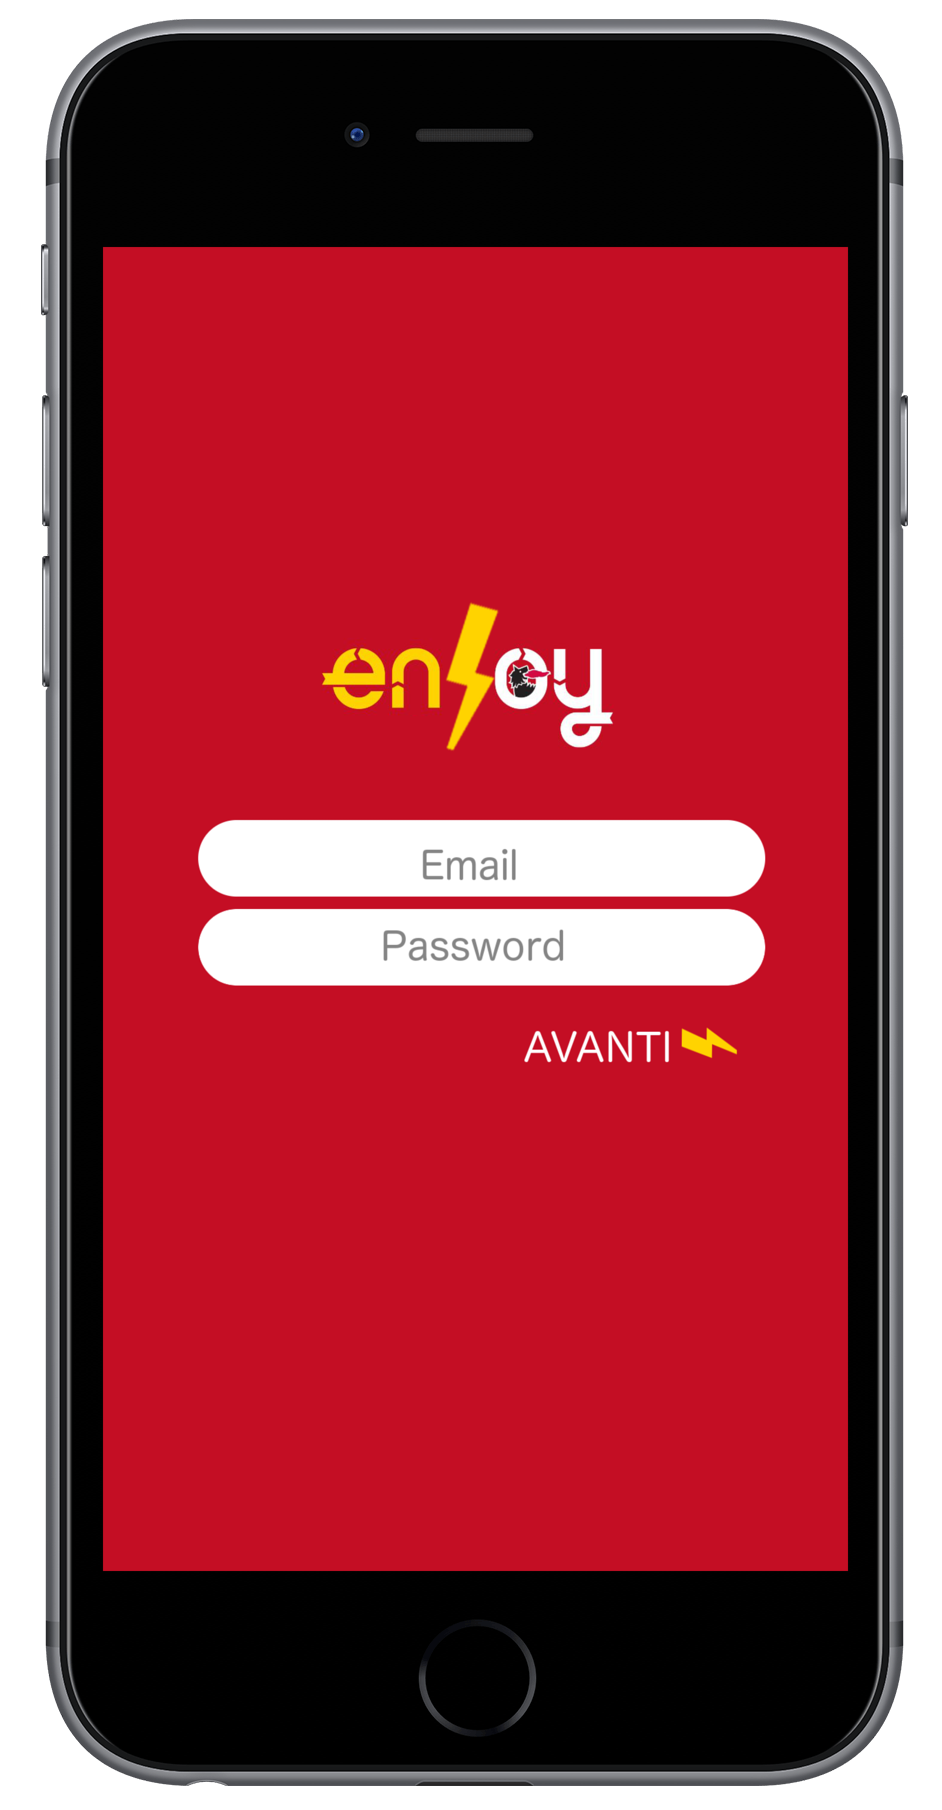
\includegraphics[width=19cm,height=19cm,keepaspectratio]{login}\\
View 1: login
\newpage
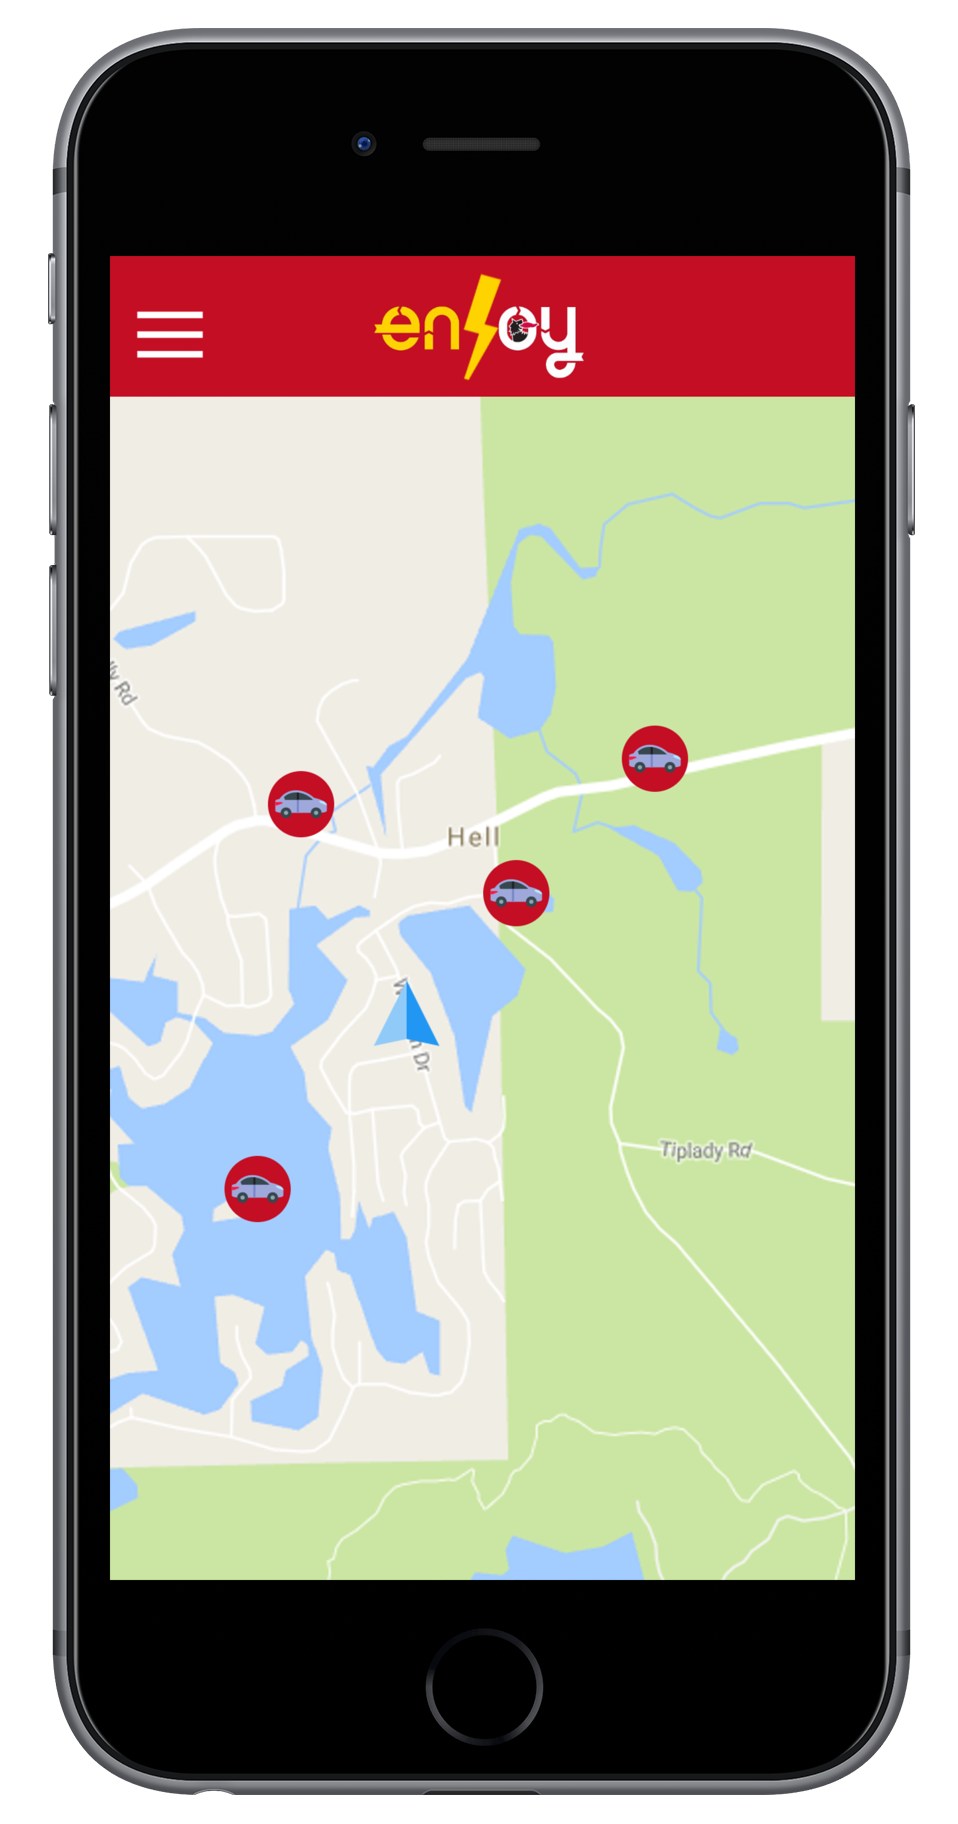
\includegraphics[width=19cm,height=19cm,keepaspectratio]{map}\\
View 2: map
\newpage
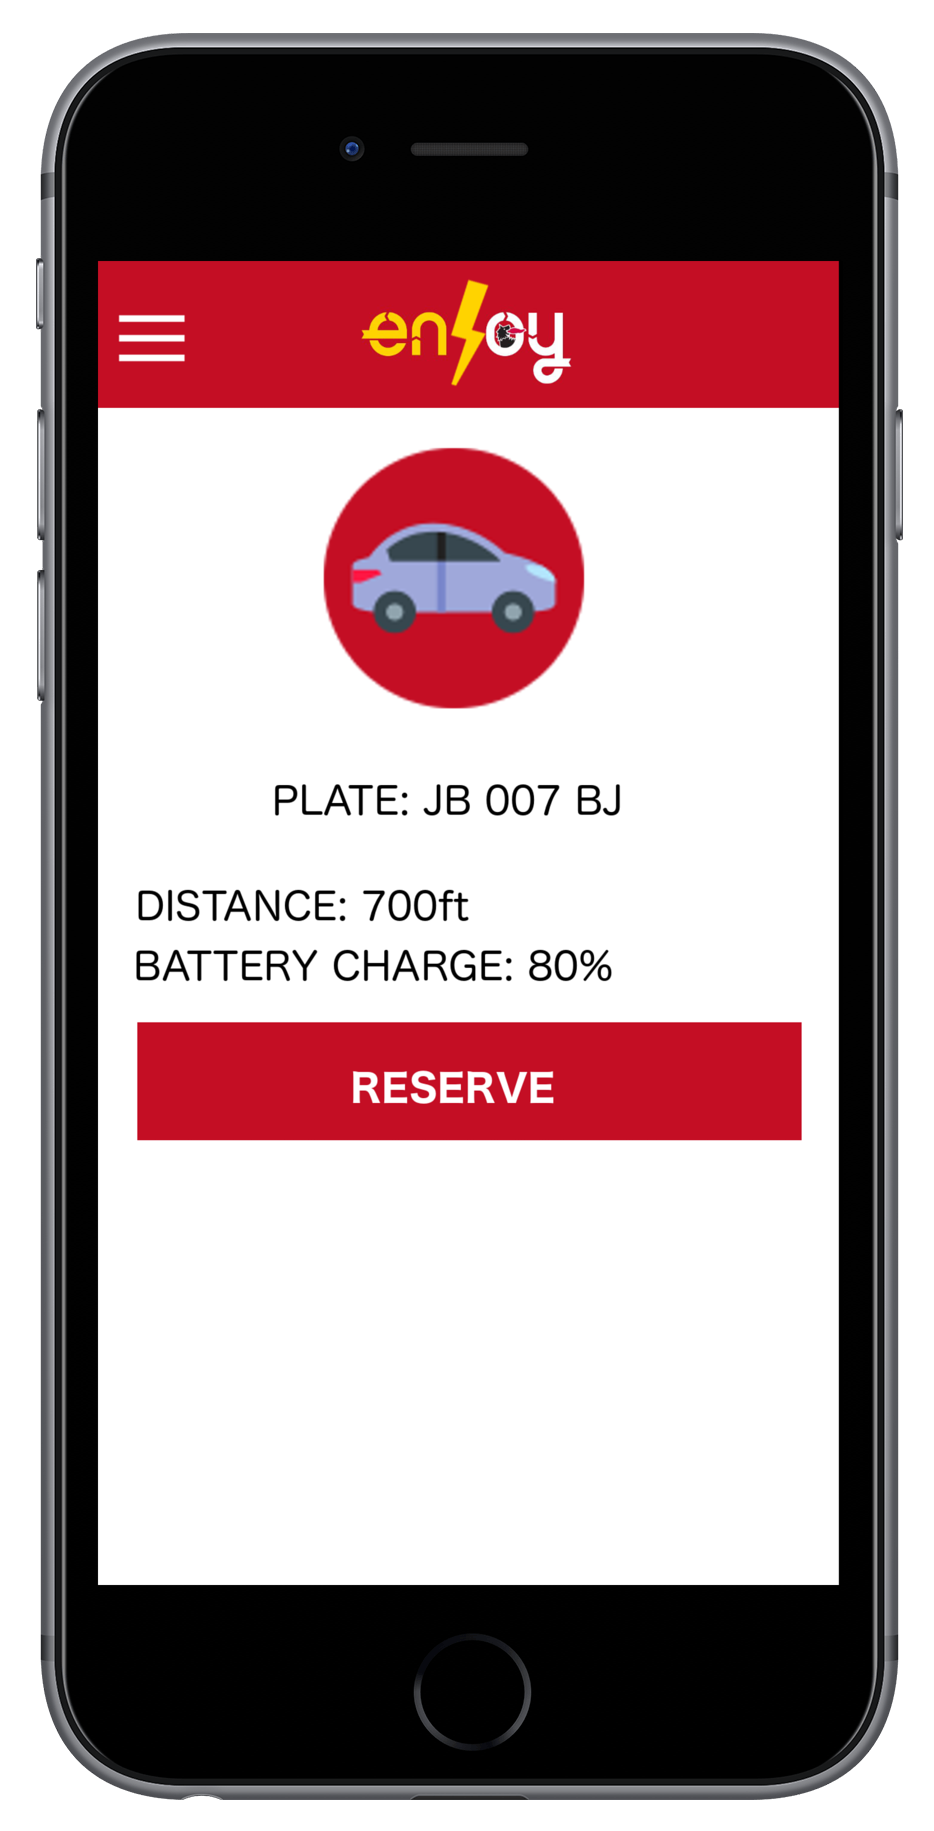
\includegraphics[width=19cm,height=19cm,keepaspectratio]{reserve}\\
View 3: reservation
\end{center}
\newpage

\subsection{Web portal}
\bigbreak
\begin{center}
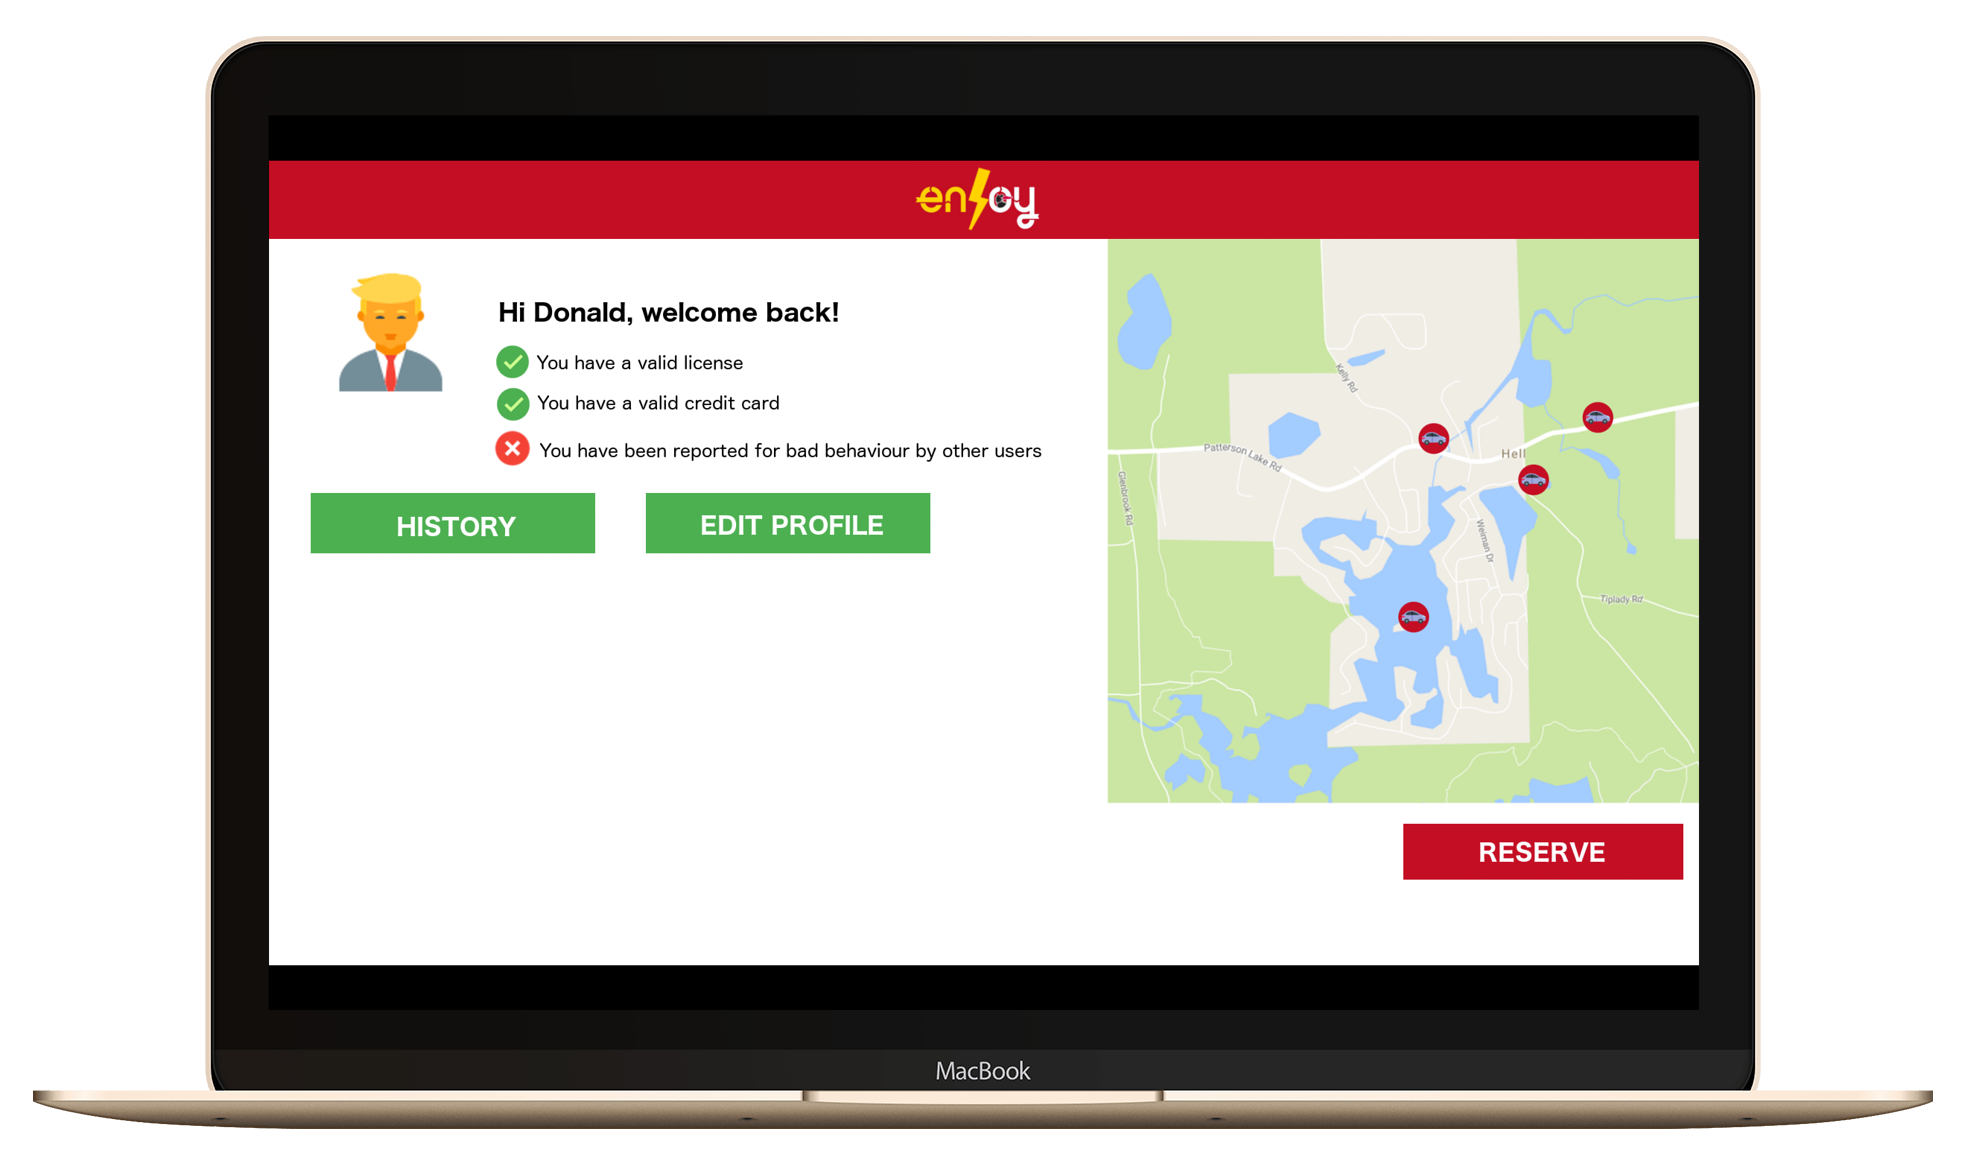
\includegraphics[width=16cm,height=20cm,keepaspectratio]{portal}
Main view
\end{center}




